% !TEX root =  paper.tex
\section{Compression of Label Volumes}

An often overlooked aspect of these segmentation datasets is how to efficiently store the label volumes.
These label volumes are often 32- or 64-bit to account for the massive number of neurons that interweave through a cubic millimeter.
Uncompressed, a cubic millimeter of segmentation data is nearly 20 petabytes.
Thus, compression techniques are needed for fast transmission and cost-efficient storage.

\subsection{Related Works}

General-purpose compression schemes~\cite{collet2016smaller,deutsch1996zlib,google2016brotli,lehmann2016liblzf,oberhumer2005lzo,pavlov2007lzma,seward1998bzip2,vandevenne2016zopfli,welch1984technique,ziv1978compression} are not optimized for this data.
With Compresso, an algorithm published in MICCAI 2017, we exploit the typical characteristics of label volumes such as large invariant regions without natural relationship between label values. 
These properties render 2D image compression schemes inadequate since they rely on frequency reduction (using e.g., wavelet or discrete cosine transform) and value prediction of pixels based on local context (differential pulse-code modulation)~\cite{roelofs1999png,skodras2001jpeg}. 
Color space optimization strategies in video codecs~\cite{aimar2005x264} also have no effect on label volumes, even though the spatial properties of a segmentation stack (\textit{z}-axis) are similar to the temporal properties of video data (time-axis). 
A compression scheme designed specifically for label volumes is part of the visualization software Neuroglancer~\cite{google2016compressed}. 
This method exploits segmentation homogeneity by creating small blocks with $N$ labels and reducing local entropy to $\log_2{N}$ per pixel. 
Lookup tables then decode the values $[0,N)$ to the original 64-bit labels.

\subsection{Method}

\begin{figure*}[t]
	\begin{center}
		\begin{minipage}{0.45\linewidth}
			\centering
			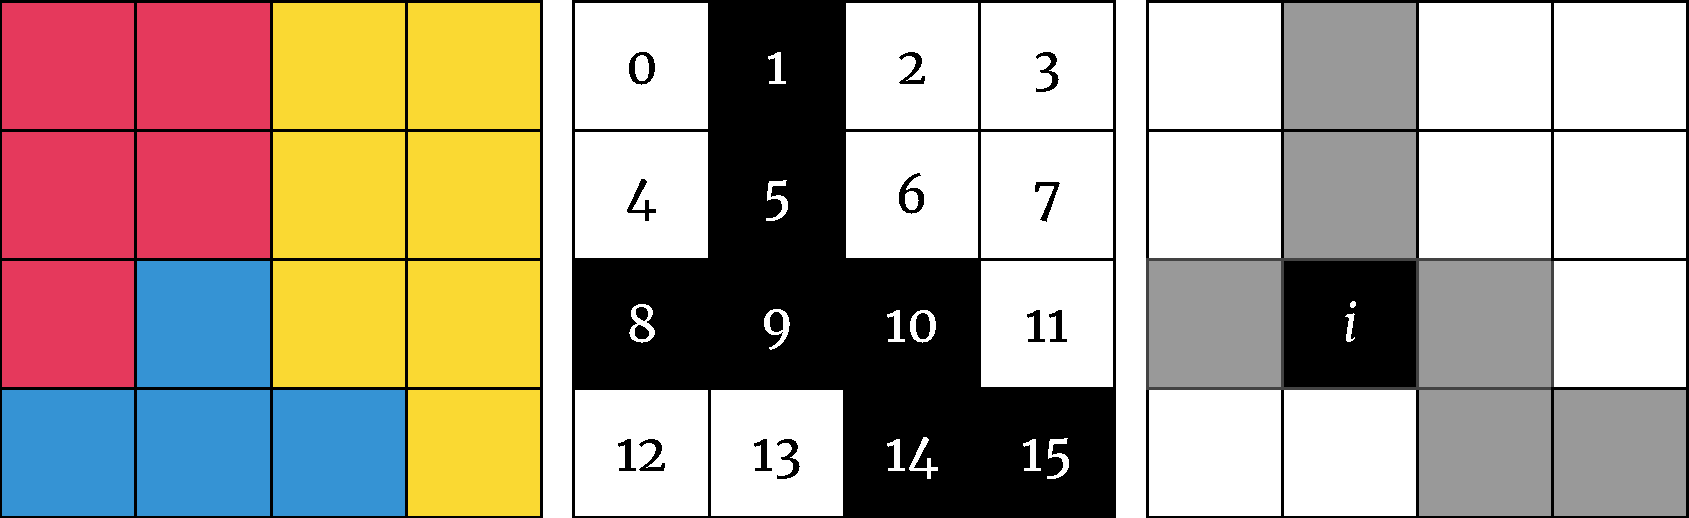
\includegraphics[width=\linewidth]{./figures/encoding_diagram_opt.pdf}
		\end{minipage}
		\hspace{0.08\linewidth}
		\begin{minipage}{0.45\linewidth}
			\centering
			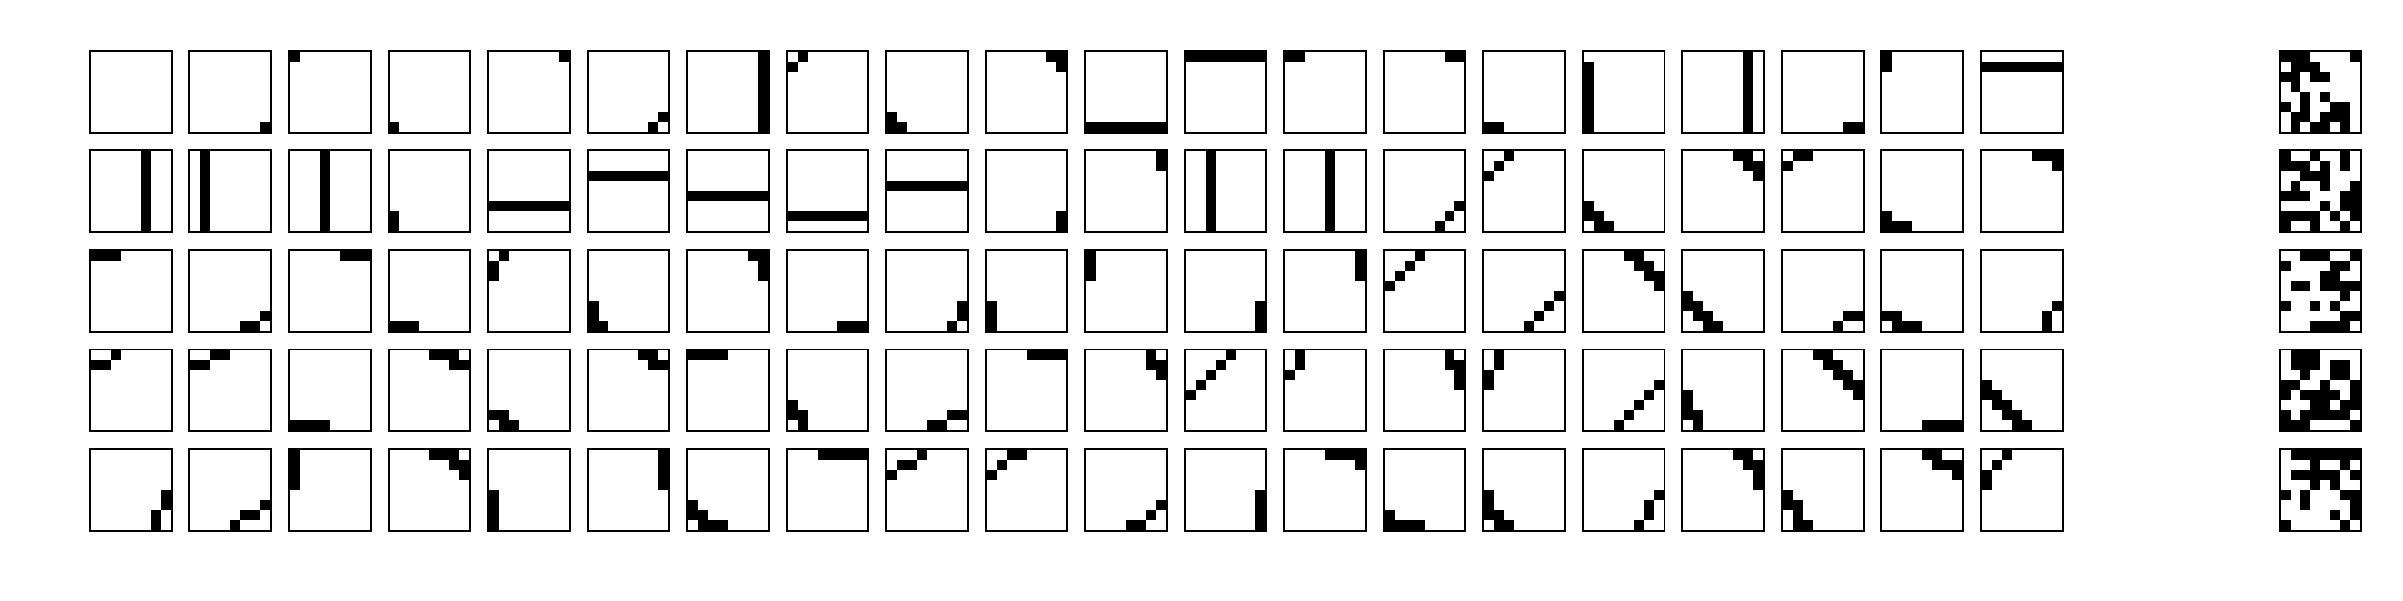
\includegraphics[width=\linewidth]{./figures/window_values.pdf}
		\end{minipage}
	\end{center}	
	\caption{Compresso works by dividing up the segmentation data into small blocks. On the left we show the intersection of three segments in a $4\times4\times1$ window. We extract a boundary map from this segmentation to transform the window into an integral value between $0$ and $2^{16} - 1$. The location $i$ requires some additional bookkeeping. On the right are the $100$ most common $8 \times 8 \times 1$ windows accounting for $\sim82\%$ of the volume on a representative dataset.}
	\label{fig:compression}
\end{figure*}


Published in MICCAI 2017, we proposed Compresso which is specifically designed for compression of EM label volumes.
Compresso works by decoupling the two important components across the image stack: per-segment shape and per-pixel label.
To encode the segment shapes, we consider the boundary pixels between two segments. 
Removing the per-pixel labels, we produce a boundary map for each slice where a pixel $(x, y, z)$ is 1 if either pixel at $(x + 1, y, z)$ or $(x, y + 1, z)$ belongs to a different segment (Fig~\ref{fig:compression}, left). 
The boundary map is divided into non-overlapping congruent 3D windows. If there are $n$ pixels per window, each window $w$ is assigned an integer $V_w \in [0, 2^n)$ where $V_w$ is defined as:

\begin{equation}
V_w = \sum_{i = 0}^{n - 1} \mathbb{I}(i) 2^i,
\end{equation}

\noindent
and $\mathbb{I}(i)$ is 1 if pixel $i$ is on a boundary and 0 otherwise. 
Figure~\ref{fig:compression}, left, shows an example segmentation with a window size of $4 \times 4 \times 1$.

A priori, each window could take any of $2^n$ distinct values, and therefore require $n$ bits to encode without further manipulation. 
However, boundaries in segmentation images are not random, and many of these values never appear. 
Indeed, we find that a small subset of high-frequency $V_w$ values accounts for most windows, allowing for significant compression. 
Figure~\ref{fig:compression}, right, shows the 100 most common windows for a representative connectomics dataset. 
These 100 frequently occurring windows account for approximately 82\% of the over 1.2 million $V_w$ values in this dataset.
Nearly all of these windows correspond to simple lines traversing through the window. 
For contrast, we also provide 5 randomly generated windows that never occur in the dataset.


We define $N$ as the number of distinct $V_w$ representing all of the windows in an image stack. 
We construct an invertible function $f(V_w) \to [0, N)$ to transform the window values into a smaller set of integers. 
For all real-world segmentations $N \ll 2^n$; however, we assume no constraint on $N$ in order to guarantee lossless compression. 
With this function, each $V_w$ requires $\log_2{N}$ bits of information to encode. 
This is fewer than the initial number of bits so long as $N \leq 2^{n - 1}$.  

So far we have focused exclusively on transforming the boundary map of an image segmentation. 
However, the per-pixel labels themselves are equally important. 
The boundary map divides each image slice into different segments. 
By design, all pixels in the same segment have the same label so we store only one label per segment for each slice. 
We use a connected-component labeling algorithm to store one label per segment \cite{he2009fast}. 
The algorithm labels all pixels clustered within a component $m$ from $M$ section labels.

Thus far, we have assumed the boundaries provide enough information to reconstruct the entire segmentation.
Pixels not on a segment boundary are easily relabeled.
However, more care is needed for pixels on the segment boundaries. 
Consider figure~\ref{fig:compression}, left, which depicts a difficult boundary to decode. 
If a boundary pixel has a non-boundary neighbor to the left or above, then that pixel merely takes on the value of that neighbor. 
However, pixel $i$ requires more care since its relevant neighbors are both boundary pixels. 
We simply just store the label values for indeterminate pixels like $i$.

To decompress the data, we first reconstruct the boundary map from the windows that we extracted.
From there, we can run the same deterministic connected-components algorithm per slice.
We can traverse through the saved labels to fill in all non-boundary labels.
To determine the per-pixel labels for every boundary pixel, we iterate over the entire dataset in raster order. 
Any boundary pixel $(x, y, z)$ with a non-boundary neighbor at $(x - 1, y, z)$ or $(x, y - 1, z)$ shares the same per-pixel label. 
If both relevant neighbors are boundaries (i.e., like pixel $i$ in Fig.~\ref{fig:compression}) we extract the value we had stored.

\subsection{Results}

Our compression scheme outperforms all existing methods.
We follow our scheme with LZMA which uses sophisticated probabilistic bit prediction strategies and achieve ratios of $700\times$ on average.
We compressed an 18 terabyte label volume of 100 microns cubed to 26.2 gigabytes, a ratio of $\sim687\times$. 
